\section{Runtime}
\label{section:noderuntime}

We define the session runtime in Svr.ts,
named after the \trole{Svr} endpoint.
It exposes a \textbf{public API}
(\cref{lst:noderuntimepublicapi})
with seams for the developer to pass in the WebSocket server 
and application logic
(i.e. their handler implementations).
It is the responsibility of the developer to construct the
WebSocket server and set it up to listen for incoming connections.
Internally, it keeps a \textit{private API}
for executing the EFSM, when all participants have 
joined the session.
The role of the public API is to manage incoming connections and
wait for all participants to join the session 
(\cref{subsection:noderuntimepublic}), before
handing off to the private API to execute the EFSM
(\cref{subsection:noderuntimeprivate}).

\begin{figure}[!h]
\begin{lstlisting}[language=javascript,tabsize=2,title=Svr.ts]
export class Svr {
	constructor(wss: WebSocket.Server,
							initialState: Implementation.S51) { ... }
	...
}
\end{lstlisting}
\captionof{lstlisting}{Public API of Session Runtime for Server Endpoint}
\label{lst:noderuntimepublicapi}
\end{figure}

\subsection{Managing Connections}
\label{subsection:noderuntimepublic}

\begin{itemize}
\item use set and partial object to keep track of pending connections
\item ws event listeners
\item forward reference that we need to manage cancellations here too
\end{itemize}

\subsection{Executing the EFSM}
\label{subsection:noderuntimeprivate}

We revisit the concept of using discriminated unions to distinguish
the type of EFSM state. The discriminated union is implemented by the
\texttt{Implementation} API which wraps the developer's
implementation of the  \texttt{Handler} API.

It is sufficient for the runtime to only discriminate the type of state
rather than the specific state. 
we can define \textit{state-specific}
details within the discriminated union


\begin{itemize}
\item implementation details delegated to the actual implementation states
\item all non-terminal states will `return' the successor implementation -- very difficult to resolve in the type-checker in the runtime (give example of what it may look like) -- solve by giving each state implementation the `advance' function to respect the event-driven nature of everything, so they can call it on completion
\item visualise the interaction between runtime and states as a sequence diagram for message passing
\item constructor binds all methods (that will be passed to other components0 to `this' because of how javascript works with respect to the scoping of `this' (give short example -- or ignore, if this is in the background for typescript)
\item advance -- use discriminated union to figure out what to pass to the state (send -- sendMessage, receive -- register)
\end{itemize}

\begin{figure}[!ht]
\centering
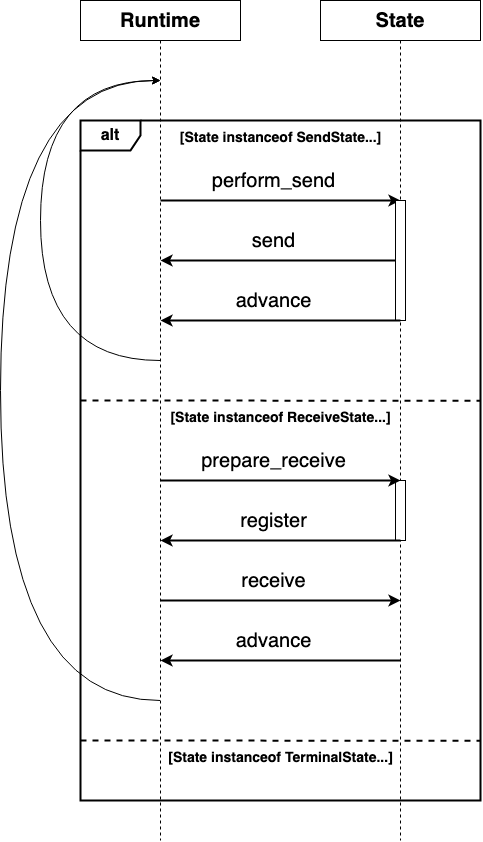
\includegraphics[width=0.5\textwidth]{NodeRuntimeEFSM}
\captionof{figure}{``Message Passing'' Abstraction of EFSM Execution for
Server Endpoints}
\label{fig:noderuntimeefsm}
\end{figure}

\subsection{Sending Messages}
Message Types are defined as interfaces, which
are represented by objects. By convention,
we serialise messages into \textit{JavaScript Object Notation}
(or JSON) \cite{json} using the built-in \texttt{JSON.stringify()}
method.

They are decoded using the same interface schema on the receiving end
using \texttt{JSON.parse()}: whilst the method return type is the
dynamic \lstonelinejs{any} type, 
we guarantee type safety by construction
as we performed the serialisation in the first place, so
we can safely interpret the deserialised content 
using a concrete type.

\subsection{Handling Message Receives}
\begin{itemize}
\item motivate the edge case that message can arrive in the websocket (in succession) before the handler is registered
\item motivate the edge case that message can arrive `out of protocol order' 
\item explain the double queue system and how that provides consistency -- emphasising that this works because of the single-threaded typescript runtime
\end{itemize}

\begin{figure}[!ht]
\centering
\begin{subfigure}[b]{0.8\textwidth}
\centering
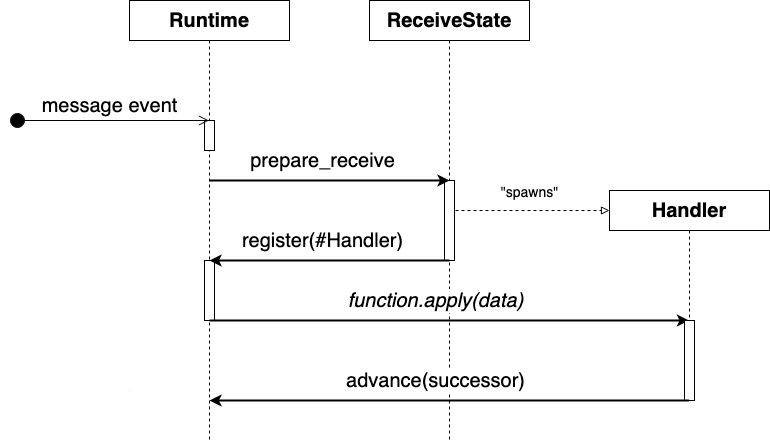
\includegraphics[width=\textwidth]{NodeRuntimeReceive2}
\caption{Message processed before transitioning to receive state}
\label{subfig:nodereceivemsgfirst}
\end{subfigure}
\hfill
\begin{subfigure}[b]{0.8\textwidth}
\centering
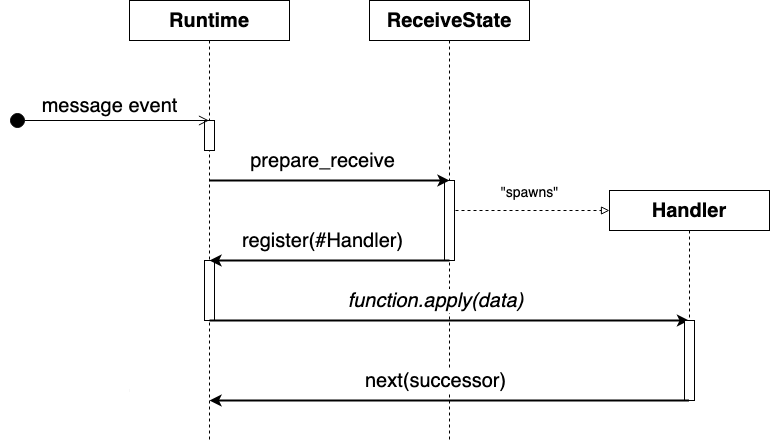
\includegraphics[width=\textwidth]{NodeRuntimeReceive1}
\caption{Message processed after transitioning to receive state}
\label{subfig:nodereceivehandlefirst}
\end{subfigure}
\captionof{figure}{Possible Orderings for Handling Message Event and Preparing
Receive State}
\label{fig:nodereceivecompare}
\end{figure}

\subsection{Handling Termination}
WebSocket connections should be closed when the session terminates,
and both the browser endpoint and the server endpoint are capable
of closing connection. As we generate code for both, we define
a convention that the browser endpoint will initiate the WebSocket
close event.